\begin{frame} \frametitle{Ним и другие игры}
	Ним с двумя кучами: {\it проигрышные} позиции — когда кучи одинаковы. \\
	Уже было сегодня. \pause

	Шоколадка, одна долька отравлена. Игроки по очереди отламывают и \\
	съедают неотравленную часть. \pause

\begin{center} \tikz[scale=0.44]{
	\fill[turnb] (3,2) rectangle ++(1,1);
	\foreach \x in {0,...,10} {
	   \foreach \y in {0,...,7} {
		\draw[gray] (\x,0) -- (\x,7) (0,\y) -- (10,\y);
	   }
	}
	\draw[thick] (0,5) -- (10,5);
	\foreach \x in {0,2,3,7} {\draw (-1,\x) -- (-0.6,\x);}
	\foreach \x in {0,3,4,10} {\draw (\x,-1) -- (\x,-0.6);}
	\draw[->,thick] (-0.8,3) -- (-0.8,7);
	\draw[->,thick] (-0.8,2) -- (-0.8,0);
	\draw[->,thick] (3,-0.8) -- (0,-0.8);
	\draw[->,thick] (4,-0.8) -- (10,-0.8);
} \end{center}
\end{frame}

\begin{frame} \frametitle{Некооперативные игры}
\begin{center}
\begin{tabular}{|c|c|c|} \hline
	& \coldescription{Split} & \coldescription{Steal} \\ \hline
	\rowdescription{Split} & \singlepayoff{5}{5} & \singlepayoff{0}{10} \\ \hline
	\rowdescription{Steal} & \singlepayoff{10}{0} & \singlepayoff{0}{0} \\ \hline
\end{tabular}\hspace{1.1cm}
\begin{tabular}{|c|c|c|} \hline
	& \coldescription{Cooperate} & \coldescription{Defect} \\ \hline
	\rowdescription{Coop.} & \singlepayoff{3}{3} & \singlepayoff{0}{7} \\ \hline
	\rowdescription{Def.} & \singlepayoff{7}{0} & \singlepayoff{1}{1} \\ \hline
\end{tabular}
\end{center}
\end{frame}

\begin{frame} \frametitle{Некооперативные игры}
\begin{center}
\begin{tabular}{|c|c|c|} \hline
	& \coldescription{Whale} & \coldescription{Fish} \\ \hline
	\rowdescription{Whale} & \singlepayoff{2}{2} & \singlepayoff{0}{1} \\ \hline
	\rowdescription{Fish} & \singlepayoff{1}{0} & \singlepayoff{1}{1} \\ \hline
\end{tabular}\hspace{1.1cm}
\begin{tabular}{|c|c|c|} \hline
	& \coldescription{Swerve} & \coldescription{Straight} \\ \hline
	\rowdescription{Swe.} & \singlepayoff{0}{0} & \singlepayoff{$-1$}{$+1$} \\ \hline
	\rowdescription{Str.} & \singlepayoff{$+1$}{$-1$} & \singlepayoff{$-1000$}{$-1000$} \\ \hline
\end{tabular}
\end{center}
\end{frame}

\begin{frame} \frametitle{Некооперативные игры}
\begin{center}
\begin{tabular}{|c|c|c|} \hline
	& \coldescription{Bach} & \coldescription{Stravinsky} \\ \hline
	\rowdescription{Bch.} & \singlepayoff{2}{1} & \singlepayoff{0}{0} \\ \hline
	\rowdescription{Str.} & \singlepayoff{0}{0} & \singlepayoff{1}{2} \\ \hline
\end{tabular}\hspace{1.1cm}
\begin{tabular}{|c|c|c|} \hline
	& \coldescription{Head} & \coldescription{Tail} \\ \hline
	\rowdescription{Hd.} & \singlepayoff{$+1$}{$-1$} & \singlepayoff{$-1$}{$+1$} \\ \hline
	\rowdescription{Tl.} & \singlepayoff{$-1$}{$+1$} & \singlepayoff{$+1$}{$-1$} \\ \hline
\end{tabular}
\end{center}
\end{frame}

\begin{frame} \frametitle{Эффективность по Парето}
	Нельзя увеличить чей-либо выигрыш без уменьшения выигрыша других.
	
	Соответствует интуитивному представлению о максимальном выигрыше. \pause

\begin{center}
\begin{tabular}{|c|c|c|} \hline
	& \coldescription{Cooperate} & \coldescription{Defect} \\ \hline
	\rowdescription{Coop.} &\cellcolor{turnb} \singlepayoff{3}{3} & \singlepayoff{0}{7} \\ \hline
	\rowdescription{Def.} & \singlepayoff{7}{0} & \singlepayoff{1}{1} \\ \hline
\end{tabular}
\end{center}
\end{frame}

\begin{frame} \frametitle{Равновесие Нэша}
	Действие каждого игрока — наилучшее возможное при известных стратегиях других игроков.
	
	Ни один участник не может увеличить свой выигрыш, если стратегии других игроков неизменны. \vspace{-0.2cm} \pause
	
\begin{center}
\begin{tabular}{|c|c|c|} \hline
	& \coldescription{Cooperate} & \coldescription{Defect} \\ \hline
	\rowdescription{Coop.} & \singlepayoff{3}{3} & \singlepayoff{0}{7} \\ \hline
	\rowdescription{Def.} & \singlepayoff{7}{0} &\cellcolor{turna} \singlepayoff{1}{1} \\ \hline
\end{tabular}
\end{center}
\end{frame}

\begin{frame} \frametitle{Существование равновесия Нэша}
\begin{center}
\begin{tabular}{|c|c|c|} \hline
	& \coldescription{Head} & \coldescription{Tail} \\ \hline
	\rowdescription{Hd.} &
		\singlepayoff{\textcolor{turna}{$+1$}}{$-1$} &
		\singlepayoff{$-1$}{\textcolor{turnb}{$+1$}} \\ \hline
	\rowdescription{Tl.} &
		\singlepayoff{$-1$}{\textcolor{turnb}{$+1$}} &
		\singlepayoff{\textcolor{turna}{$+1$}}{$-1$} \\ \hline
\end{tabular}
\end{center} \medskip \pause

Иногда равновесия Нэша не существует в чистых стратегиях. \\
Но оно всегда есть в {\it смешанных стратегиях.}
\end{frame}

\begin{frame} \frametitle{Пиар «Математики НОН-СТОП»}
\begin{center}
	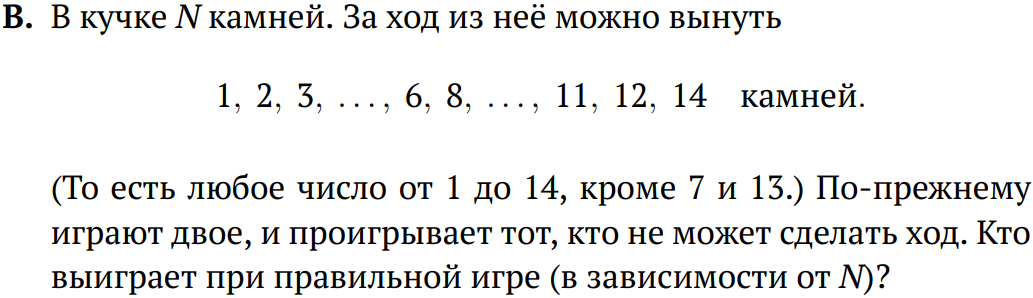
\includegraphics[width=0.7\textwidth]{img/mnsgame} \vspace{1cm}
	
	{\large\tt mathnonstop@timeforscience.ru}
\end{center}
\end{frame}
